%%%%%%%%%%%%%%%%%%%%%%%%%%%%%%%%%%%%%%%%%
%Final Year Project Report Bachelor of Engineering
% LaTeX Template

% Authors:
% John Davies, John.Davies@glasgow.ac.uk
% VAN DARKHOLME & Huang Yifan, 2288862h@student.gla.ac.uk 
% Bernd Porr, bernd.porr@glasgow.ac.uk

%----------------------------------------------------------------------------------------
%	PACKAGES AND OTHER DOCUMENT CONFIGURATIONS
%----------------------------------------------------------------------------------------

\documentclass[
12pt, % The default document font size, options: 10pt, 11pt, 12pt
oneside, % Two side (alternating margins) for binding by default, uncomment to switch to one side
singlespacing, % Single line spacing, alternatives: onehalfspacing or doublespacing
parskip, % Uncomment to add space between paragraphs
]{article} % The class file specifying the document structure

\usepackage{geometry}

\usepackage[utf8]{inputenc} % Required for inputting international characters
\usepackage[T1]{fontenc} % Output font encoding for international characters
\usepackage{mathptmx}%%% Use the Times font by default%%%

\usepackage{color}%U can change font color

\usepackage[scaled]{helvet} % helvetica for sanserif, scaled 95% by default

\usepackage{courier}  % for typewriter text

\usepackage{textcomp} % lots of useful symbols

\usepackage{graphicx}  % inclusion of graphics files
\graphicspath{{figures/}{./}}

\usepackage{hyperref}

\usepackage{wrapfig}   % For better figures
\usepackage{physics}   %For Partial Derivatives
\usepackage{amsmath}   % for aligning formulae 
\usepackage{amssymb}
\usepackage[rightcaption]{sidecap}
\usepackage{multicol}
\usepackage{mathtools,siunitx,array,mleftright}

\usepackage[skip=2pt]{caption}
\usepackage{subcaption}
\usepackage{blindtext}

\DeclareCaptionFormat{myformat}{\fontsize{11}{6}\selectfont#1#2#3}
\captionsetup{format=myformat}

\urlstyle{format=myformat}


\newcommand{\thesistitle}{Biologically inspired UAV} % Your thesis title, this is used in the , print it elsewhere with \thesistitle
\newcommand{\GUID}{2391076M}% Your GUID, this is used in the , print it elsewhere with \GUID
\newcommand{\student}{Oscar \textsc{Meunier}} % Your name, this is used in the title page and abstract, print it elsewhere with \student
\newcommand{\firstsupervisor}{\textcolor{red}{\tiny Keep blank before hardcopy submission}} % Your 1st supervisor's name, this is used in the title page, print it elsewhere with \firstsupervisor. YOU NEED TO KEEP BLANK FOR MOODLE SUBMISSION BUT PUT THE NAME BEFORE HARDCOPY SUBMISSION.
\newcommand{\secondsupervisor} {\textcolor{red}{\tiny Keep blank before hardcopy submission}}% Your 2nd supervisor's name, this is used in the title page, print it elsewhere with \secondsupervisor. YOU NEED TO KEEP BLANK FOR MOODLE SUBMISSION BUT PUT THE NAME BEFORE HARDCOPY SUBMISSION.

%----------------------------------------------------------------------------------------
%	OTHER INFORMATION 
%----------------------------------------------------------------------------------------

\newcommand{\degree}{Mechanical Engineering with Aeronautics} % Your degree name, this is used in the title page and abstract, print it elsewhere with \degree
\newcommand{\subject}{Electric & Electronic Engineering} % Your subject area, this is not currently used anywhere in the template, print it elsewhere with \subject
\newcommand{\keywords}{} % Keywords for your thesis, this is not currently used anywhere in the template, print it elsewhere with \keywords
\newcommand{\university}{\href{https://www.gla.ac.uk/}{GU}} % Your university's name and URL, this is used in the title page and abstract, print it elsewhere with \university
\newcommand{\department}{\href{https://www.gla.ac.uk/schools/engineering/}} % Your department's name and URL, this is used in the title page and abstract, print it elsewhere with \department


\renewenvironment{abstract}{
	\section*{Abstract}
	\bigskip
	\addcontentsline{toc}{section}{Abstract}}{\clearpage}

\newenvironment{acknowledgement}{
	\section*{Acknowledgements}
	\bigskip
	\addcontentsline{toc}{section}{Acknowledgements}}{\clearpage}


\geometry{
	paper=a4paper, % Change to letterpaper for US letter
	inner=6em, % Inner margin
	outer=6em, % Outer margin
	bindingoffset=0em, % Binding offset
	top=6em, % Top margin
	bottom=6em, % Bottom margin
	%showframe, % Uncomment to show how the type block is set on the page
}
\hypersetup{colorlinks=true,linkcolor=black,citecolor=black}% Remove read block in the content
\AtBeginDocument{
\hypersetup{pdftitle=\thesistitle} % Set the PDF's title to your title
\hypersetup{pdfauthor=\student} % Set the PDF's author to your name
\hypersetup{pdfkeywords=\keywords} % Set the PDF's keywords to your keywords
}



\begin{document}


\pagestyle{plain} % Default to the plain heading style until the thesis style is called for the body content

%----------------------------------------------------------------------------------------
%	TITLE PAGE
%----------------------------------------------------------------------------------------

\begin{titlepage}
\begin{center}

\textsc{\Large Final Year Project Report\\Bachelor of Engineering
}\\[2cm] % Thesis type

{\huge \bfseries \thesistitle\par}\vspace{3cm}% Thesis title

\begin{minipage}[t]{0.4\textwidth}
\begin{flushleft} \huge
Student:\\
\vspace*{.02\textheight}
GUID:\\
\vspace*{.02\textheight}
$1^{st}$\, Supervisor:\\
\vspace*{.02\textheight}
$2^{nd}$ Supervisor:\\
\end{flushleft}
\end{minipage}
\begin{minipage}[t]{0.4\textwidth}
\begin{flushright} \huge
\student\\
\vspace*{.02\textheight}
\GUID\\
\vspace*{.02\textheight}
\firstsupervisor\\
\vspace*{.02\textheight}
\secondsupervisor\\
\end{flushright}
\end{minipage}\\[3cm]

 
\vfill

{\huge 2021-2022}\\[2cm] % Date
%\includegraphics{Logo} % University/department logo - uncomment to place it
 
\end{center}
\end{titlepage}


\pagenumbering{roman}
%----------------------------------------------------------------------------------------
%	DECLARATION PAGE
%----------------------------------------------------------------------------------------
\renewcommand{\arraystretch}{1.3}

%----------------------------------------------------------------------------------------
%	ABSTRACT PAGE
%----------------------------------------------------------------------------------------

\begin{abstract}
This Project uses reinforcement learning (RL) to develop flocking behaviour in drones to organise groups of UAVs using biologically inspired behavioural models. This explores how a multi-agent model is simulated and how the loss function can be constructed to achieve emergent behaviour focusing on how the reward function can be scaled with N agents. The model used is an actor-critic model as this allows for continuous action and observation states. The 2D environment is constructed by layering potential field functions and boid flocking behaviour. The agent controls drones using gains that amplify certain behaviours and is trained to maximise long term cumulative reward. The reward function is constructed using variations on the exponential function to flock and arrive within a certain number of steps. 
As a result, flocking behaviour was achieved and can be scaled although computational resources meant that this was limited. Issues in the behaviour do arise however where some drones fail to arrive at the destination, prioritising flocking. This is most likely due to reward function design as well as some limitations in the simulation. This dissertation demonstrates how reinforcement learning can be used with multi-vehicle UAV applications. By changing the (RL) structure to a more suitable multi-agent particle environment such as the ones available in the openAI database this could be applied at different scales whilst being much more conservative with computational requirements.
\end{abstract}

%----------------------------------------------------------------------------------------
%	ACKNOWLEDGEMENTS
%----------------------------------------------------------------------------------------

\begin{acknowledgement}
I would like to express my gratitude to my advisor, Dr Kevin Worrall for providing me with advice and steering me towards information that would prove essential to this dissertation. Dr Worrall has also advised me further and is one of the reasons I have chosen to pursue a MSc of robotics and artificial intelligence at the university of Glasgow.\\
Dr Dezong Zhao's, my professor for autonomous guided systems has also been an enormous help in creating the model that was used in this dissertation. I would like to thank him for his clear and well-formulated lectures from which I have derived a lot of the code for the simulation.\\
I would also like to thank Daniel Shiffman, the author of the nature of code, who's  tutorials have been an enormous help in learning how to code multiple agents efficiently.\cite{cod2}\\
In addition, I would like to thank Dr Lex Fridman, a professor of the university of MIT, who has provided his lectures on deep neural networks for free. \cite{lex1}\\

\end{acknowledgement}

%----------------------------------------------------------------------------------------
%	LIST OF CONTENTS
%----------------------------------------------------------------------------------------
\tableofcontents % Prints the main table of contents
\pagebreak
%----------------------------------------------------------------------------------------
%	THESIS CONTENT - SECTIONS
%----------------------------------------------------------------------------------------

\pagestyle{plain} % Return the page headers back to the "thesis" style

\pagenumbering{arabic}
% Include the sections of the thesis as separate files from the sections folder
% Uncomment the lines as you write the sections

\section{Introduction}
In recent decades UAV technology is becoming increasingly more accessible as today’s manufacturing enables cheaper, smaller, and more powerful electric motors. Companies such as Drone up\cite{com1}, Wing\cite{com2} and DHL\cite{com3} are developing autonomous drones to enable companies to deliver packages. Other projects such as Europe's \emph{SKYOPENER} \cite{com4} aim to expand civilian applications of Remotely Piloted Aircraft Systems (RPAS).\\
There is some discussion over the efficiency of drones in comparison to electric vehicles. A 2019 study \cite{eff1} found that switching entirely to drones would not be desirable in terms of total efficiency but could be useful in a last-mile approach for light and short distance deliveries. \emph{RAND Corporation}, a research organization,\cite{eff2} estimates that if 20\% of deliveries were replaced by drones this could decrease diesel consumption of the United Parcel Service (UPS) by 5.7\%, reducing the carbon footprint due to trucking as they are converted to electric substitutes.

\vspace{0.5cm}
\begin{wrapfigure}{h}{0.32\textwidth}
\centering
    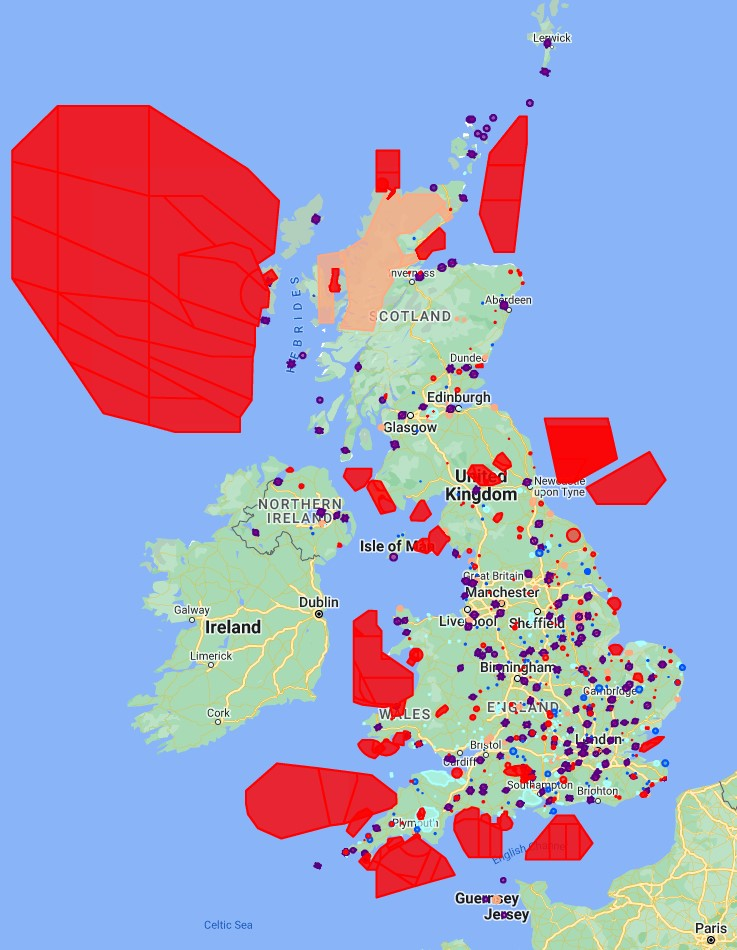
\includegraphics[width=0.3\textwidth]{figures/NoFly.jpg}\hfill
    \caption{UK restricted airspace}
    \label{fig:nofly}
\end{wrapfigure}

Drone flight is already somewhat controlled via legislation, figure \ref{fig:nofly} shows restricted zones in the UK\cite{res1}. One can see how this would become a complex guidance control problem especially if a drone needs to interact with other UAVs, with which it does not have direct communication.   A city council or other similar entity might want more localised control over which airspace is used and when this is the case. As the drone industry expands and evolves so does the control problem. By using reinforcement learning drones might be able to adapt. 

This essay looks at a hypothetical future where drones are used on a much larger scale. Being as easily manoeuvrable as they are and some drones having a range of up to 100km \cite{far1} (although high-end consumer drones manage about 10-15km \cite{far2}) the risk of malicious use of drones is a threat that should not be taken lightly.\cite{ter1} If drones are used more frequently, we may be dependent on the network they provide. Cyber-attacks could be a way of causing havoc and affecting supply chains. For this reason, measures should be prepared to mitigate these risks to the maximum extent. Anti-drone technology is available\cite{ter2} and companies such as D-fend \cite{ter3} are already working towards the solution although a full consensus is yet to be arrived at as different systems each has risks and limitations\cite{ter4}.

While fixed-wing UAVs benefit from flocking in the same way as migratory birds do quad-copter drones do not. Therefore, this application focuses on how to control drone traffic of general UAVs. As it allows for a general agent to be created which can adapt in real-time. If a general agent can be created this could reduce the problem of scaling as all computing could be achieved by individuals.
In this investigation, a reinforcement learning agent will be trained to optimise drone traffic by layering boid flocking behaviour and potential functions. This will mean that multiple agents will come to a general consensus on a trajectory through sensing the aggregate of proximal agent headings and positions.
\clearpage 

%body
%FIGURE IMPROVEMENTS- Steering force, Drone flocking


\section{Guidance methods}
In this simulation, drones will be controlled using a combination of boid flocking behaviour\cite{boid1} and artificial potential field functions\cite{con1}.

\subsection{Potential field functions}
In a similar fashion to conservative forces such as gravity and electrostatic force, the guiding force acting on each drone can be represented as a potential field function \textbf{\(U\)}. An important property of conservative forces is:

\begin{equation}
    \vec{F} = -\Delta U = -\begin{bmatrix}\pdv{U}{x} & \pdv{U}{y}\end{bmatrix}^T
    \label{equ:force}
\end{equation}
\\
We can define the attractive potential \(U_a\) of a point as:

\begin{equation}
    U_a=\frac{1}{2}K_a\rho_a^2
    \label{equ:AtP}
\end{equation}
\noindent
       Where, \(\rho_a = \sqrt{(x - x_a)^2 + (y - y_a)^2}\) is the distance to that point and \(K_a\) is the attractive constant. This is depicted in figure \ref{fig:Atractivepot} where \(x_a\) and \(y_a\) are the coordinates of the destination and \(x\) and \(y\) are coordinates of the drone. This will be used as the guiding force towards individual destinations. Using equations \ref{equ:force} and \ref{equ:AtP} the attractive force can be found as:
       \[\vec{F_a}=\nabla U_a = \nabla \left(\frac{1}{2}K_a\Big[(x - x_a)^2 + (y - y_a)^2\Big]\right)\]
       so,
       \begin{equation} \label{equ:AtractiveForce}
       \begin{split}
                &  F_{ax} = K_a(x_a - x) \\
                &  F_{ay} = K_a(y_a - y)
        \end{split}
       \end{equation}
       which can be represented as:
       \begin{equation}
           \vec{F}_a = K_a\vert\vec{p}_{a} - \vec{p}_{d}\vert
       \end{equation}
       \noindent
       Where $\vec{p_{a}}$ and $\vec{p_{d}}$ are the attractive and drone position vectors respectively. For later simplification $|\vec{p_{a}} - \vec{p_{d}}| = \vec{V}_E$. Where $\vec{V}_E$ is the desired velocity vector in the direction of the potential field.
       \begin{figure}[h]
    \centering
    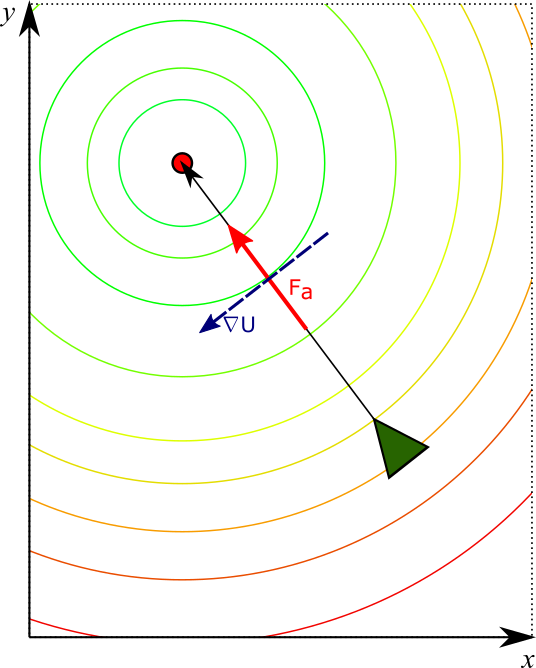
\includegraphics[width=0.25\textwidth]{figures/AtractiveForce.png}
    \caption{Potential field of destination of one drone}
    \label{fig:Atractivepot}
\end{figure}

\noindent
From figure \ref{fig:Atractivepot} it can be seen that the attractive potential is such that the force always acts towards the destination.
\clearpage

\subsection{Steering Force}

\begin{wrapfigure}{r}{0.3\textwidth}
    \begin{center}
    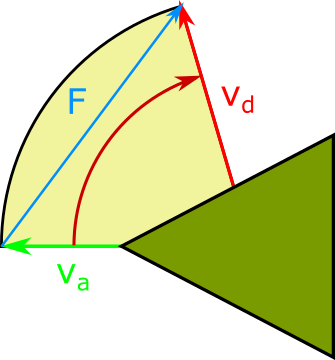
\includegraphics[width=0.2\textwidth]{figures/PropNav.png}
    \end{center}
    \caption{Steering force}
    \label{fig:PropNAv}
\end{wrapfigure}

Steering force is what gives autonomous agents the ability to steer via their own coordinate system. This simple guidance law established by Craig Reynolds \cite{boid4} is the difference between the actual velocity \(\vec{v_a}\) of the drone and the desired velocity heading \(\vec{v_d}\) determined by the behavioural model. So the steering force is:

\begin{equation}
    \vec{F} = K(\vec{v_a} - \vec{v_d})
\end{equation}

Where K is a gain which determines the weight of a specific behaviour.

\subsection{Flocking behaviour} \label{flock}
The flocking behaviour that will be introduced is from Craig Reynold's work on boids \cite{boid1} and model formulae are established from derivative work  \cite{boid3}. This uses boid steering behaviour to mimic the aggregate motion of group herding/flocking dynamics. This motion that we recognise as flocking depends upon a localised perception of the world as in nature where, in large flocks or herds, individuals are only aware of proximal members.
The local flock is determined by the perception radius, $r_p$, of each individual. Flockmates will be used to refer to  drones within the perception radius of each subject drone as demonstrated in figure \ref{fig:Flocking}. 

\begin{figure}[h]
    \centering
    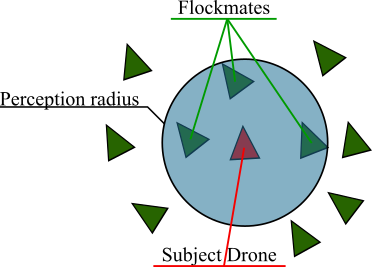
\includegraphics[width=0.5\textwidth]{figures/Flocking.png}
    \vspace{0.2cm}
    \caption{Drone flocking}
    \label{fig:Flocking}
\end{figure}

The direction and speed of every subject drone \(A\) at position \(\vec{p}_{A}\) depends on the direction and speed of all flock-mates within its perception radius \(r_p\). So for all other drones in with a position \(\vec{p_X}\) if:

\begin{equation}
    \Vert\vec{p}_{X}-\vec{p}_{A}\Vert\leq r_{p}
    \label{equ:per}
\end{equation}



\noindent


Then the drone is a flock-mate and therefore is a member of the set ${\cal{F}}_i \subset\{1,2,...N\}/\{i\}$. Otherwise, it is ignored. ${\cal{F}}_i$ then represents the set of all drones that agent $i$ is aware of.\hfill\\
\clearpage
\noindent
The localised flocking will be comprised of 3 steering behaviours that describe how the drone moves based on the velocities and positions of flock-mates. Note that || denotes a scalar vector magnitude and | is a directional vector. The behaviours are as follows:

\subsubsection{Separation}
The entity must keep its distance from other drones to avoid collisions. To achieve this the drone manoeuvres away from other drones with a force inversely proportional to the distance between them:

\begin{equation}
\vcenter{\hbox{\begin{minipage}{5cm}
\centering
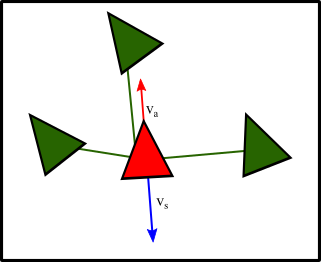
\includegraphics[width=4.5cm]{figures/Separation.png}
\captionof{figure}{Separation force}
\end{minipage}}}
\qquad\qquad
\begin{aligned}
\vec{v}_{s_i}=\sum\limits_{j={\cal{F}}_i}{\vert \vec{p}_{j}-\vec{p}_{i}\vert \over \Vert\vec{p}_{j}-\vec{p}_{i}\Vert }\\ 
so,\hspace{0.2cm}\vec{F_S}_i = K_s\vec{V}_{DS} = K_s(\vec{v}_{a_i} - \vec{v}_{s_i}) 
\end{aligned}
\label{equ:sep}
\end{equation}


\subsubsection{Alignment}
By taking the average of all velocity vectors of its flock-mates, each drone steers into alignment with its flock-mates. The flock comes to a consensus of heading through velocity matching.\hfill

\begin{equation}
\vcenter{\hbox{\begin{minipage}{5cm}
\centering
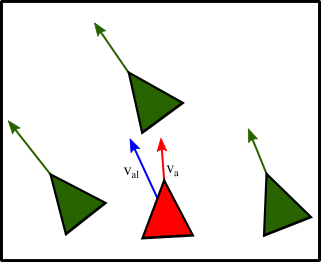
\includegraphics[width=4.5cm]{figures/Alingment.png}
\captionof{figure}{Alignment force}
\end{minipage}}}
\qquad\qquad
\begin{aligned}
\vec{v}_{al_i}=\sum\limits_{j={\cal{F}}_i}\vec{v_j}\\
so,\hspace{0.2cm}\vec{F_{Al_i}} = K_{al}\vec{V}_{DA} = K_{al}(\vec{v}_{a_i} - \vec{v}_{al_i})
\end{aligned}
\label{equ:al}
\end{equation}


\subsubsection{Cohesion}
This is what keeps the flock grouped together. Members of the flock move towards the average position of the flock. This includes the subject drone position.

\begin{equation}
\centering
\vcenter{\hbox{\begin{minipage}{5cm}

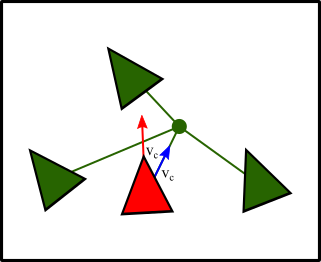
\includegraphics[width=4.5cm]{figures/Cohesion.png}
\captionof{figure}{Cohesion force}
\end{minipage}}}
\qquad\qquad
\begin{aligned}
\vec{v}_{c_i}= {\vec{p}_{i} + {{\sum\limits_{j={\cal{F}}_i}\vec{p}_{j}}}}\\ 
so,\hspace{0.2cm}\vec{F_{C_i}} = K_c\vec{V}_{DC}= K_c(\vec{v}_{a_i} - \vec{v}_{c_i})
\end{aligned}
\label{equ:coh}
\end{equation}

\noindent
\(K_s\), \(K_{al}\) and \(K_c\) are the separation gain alignment gain and cohesion gain respectively. They drive the flocking behaviour of the agent by increasing the magnitude of velocity vectors $\vec{V}_{DS}$, ${al}\vec{V}_{DA}$ and $\vec{V}_{DC}$.
\clearpage


\begin{wrapfigure}{r}{0.25\textwidth}
\centering
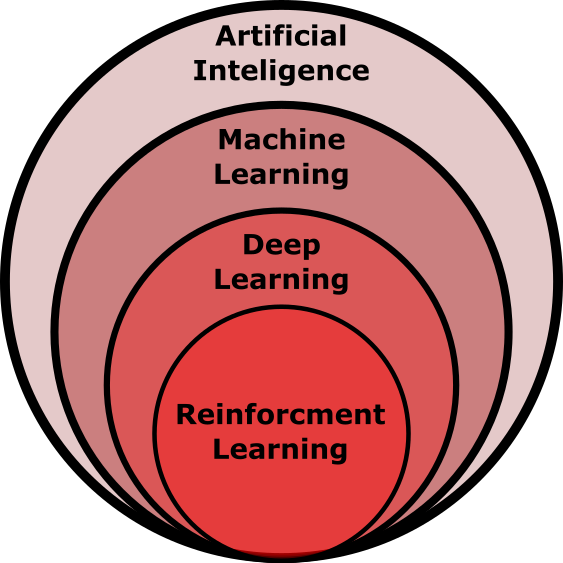
\includegraphics[width= 0.25\textwidth]{figures/AI Subsets.png}
\caption{Reinforcement learning subset}
\label{fig:sub}
\end{wrapfigure}

\section{Machine learning problem}
Machine learning is a subset of artificial intelligence, and deep learning is a subset of Machine learning. Deep learning classifies machine learning that uses deep neural networks. The neural network used in this scenario is an actor-critic, reinforcement learning (RL) approach
that reaches an optimal solution through the simulation of multiple episodes.\cite{rl2}

\subsection{Neural networks and deep learning}

  Artificial neural networks (ANN) are comprised of the input layer, hidden layers and the output layer. There can be many hidden layers constructed using perceptrons, the building block of an ANN, that map the inputs to the outputs. ANNs can have multiple inputs and outputs behaving as a MIMO controller and can map highly nonlinear input functions to any output signal. This is why they are commonly termed universal approximators.
\begin{figure}[h]
\centering
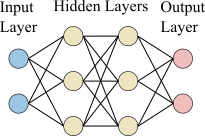
\includegraphics[width= 0.3\textwidth]{figures/NeuralNetwork.png}
\caption{Artificial Neural Network}
\label{fig:neu}
\end{figure}

\subsubsection{Perceptron}
The perceptron, shown in figure \ref{fig:per} is the activation function of a weighted sum.
\begin{figure}[h]
\centering
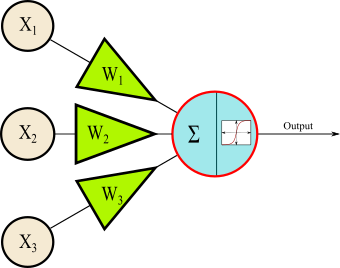
\includegraphics[width= 0.25\textwidth]{figures/Perceptron.png}
\caption{Perceptron}
\label{fig:per}
\end{figure}


\noindent
So with inputs and weight are:

\[\textbf{\textit{x}} = [x_1,x_2,...,x_k] , \textbf{\textit{w}} = [w_1,w_2,...,w_k]\]

\noindent
then, 

\[\textbf{\textit{x}} \cdot \textbf{\textit{w}} + b = 0\]
\noindent
The hidden layers made up of perceptrons change their weights and biases through back-propagation in the direction suggested by the loss function covered later on. In this case, the actor-critic network is used.

\clearpage
\subsubsection{Activation function}
An activation function is used since this allows the agent to map complex relationships of output and input. It can vary but, in this case, the sigmoid function is used as it can map continuous functions from \(0\) to \(1\).

\begin{equation}\centering
\vcenter{\hbox{\begin{minipage}{7cm}
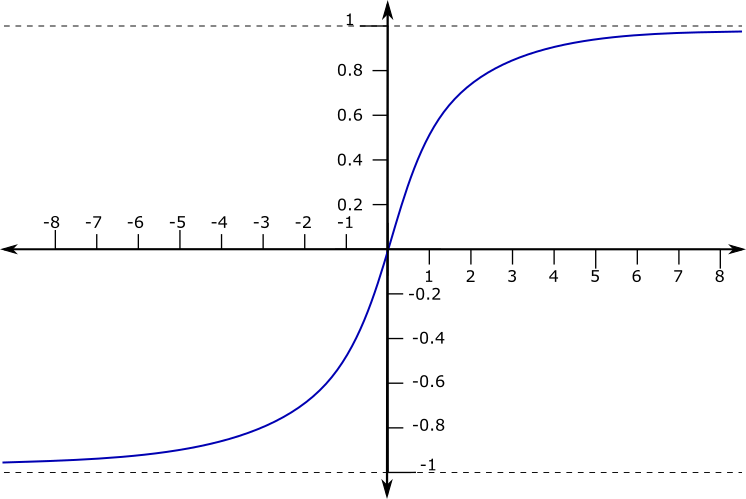
\includegraphics[width=5cm]{figures/Sigmoid.png}
\captionof{figure}{Sigmoid activation Function}
\end{minipage}}}
\qquad\qquad
\begin{aligned}
\sigma(z) = {1\over{1+e^{-z}}}
\end{aligned}
\end{equation}

As the input goes from \(-\infty\) to \(+\infty\) the output ranges from \(0\) to \(1\). This means large differences in the input are normalised which allows the network to learn highly non-linear functions.
\clearpage
\subsection{Reinforcement Learning}
\begin{wrapfigure}{r}{0.4\textwidth}
  \begin{center}
    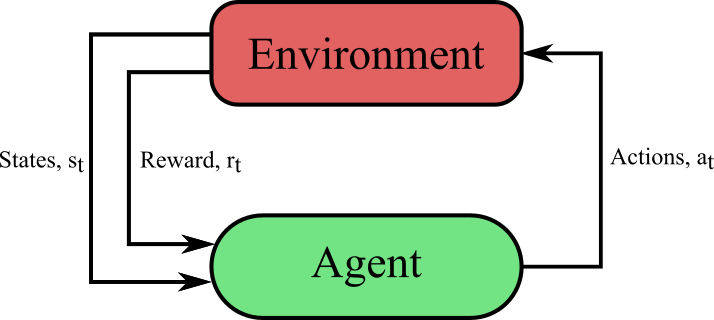
\includegraphics[width=0.4\textwidth]{figures/EnvironmentAgent.png}
    \end{center}
    \caption{Reinforcement learning Agent}
    \label{fig:Actor agent}
\end{wrapfigure}

Reinforcement learning (RL) \cite{rl1} is used to optimise complex or unpredictable control. The agent interacts with an environment to maximise reward. At each discrete time step $t$, with a given state $s \in S$ the agent chooses an action $a_t \in A$ with respect to the policy function $\pi : S \xrightarrow{} A$. The agent then receives a reward $r_{t+1}$ and a new state $s_{t+1}$ for that action\cite{ac1}. This model is known as a Markov Decision Process(MPD)\cite{mar1}, which means the agent acts in a discrete, stochastic, sequential environment.

\subsubsection{Policy}
Policy \begin{math}\pi_\theta(s_t,a_t)\end{math} can be either Stochastic or deterministic:

\begin{itemize}
\item
\textbf{Deterministic} -
A policy is deterministic if there is a clear action for any state. This will not explore new options and is referred to as greedy. This would be a pre-trained agent which has a consistent behaviour.

\item
\textbf{Stochastic } -
This policy means that there is some statistical element of variation is included.  $ \pi_\theta(s_t,a_t) $ represents the conditional probability density at $a_t$ associated with the policy.\cite{ac2} 

\end{itemize}

In this case, the policy \begin{math}\pi_\theta(s_t,a_t)\end{math} behaves stochastically with the MPD environment such that:

 \[s_0,a_0,r_1,s_1,a_1,r_2, ... ,s_{k-1},a_{k-1},r_n,s_k\]

The policy $\pi_\theta(s_t,a_t)$ is a neural network with policy parameters $\theta$ which are initialised at arbitrary values. The policy parameter are then changed using the policy gradient theorem covered later\cite{rl2} to maximise long cumulative reward.
 
\subsubsection{Reward}

The return at time step t is is defined as the discounted sum of rewards:

\[r_t^\gamma =  r_t + \gamma r_{t+1} +\gamma^2 r_{t+2} + ... +\gamma^{k-t} r_k\]

\noindent

Return is often expressed as $G_t$ and can be represented as:

\begin{equation}
     G_t = r_t^\gamma = \sum_{k =  t}^T\gamma^{k-t}r(s_k,a_k)
     \label{equ:rew}
\end{equation}

Where discount factor $0< \gamma < 1$  determines the priority of the short term rewards. This  pushes the agent to finish the simulation faster as it decreases since the short term reward is less valuable than long term reward.

\subsubsection{Value function and bellman optimality}
A value function is defined as the estimated total discounted reward. In this case, a Q-actor-critic network is used which means the \textbf{state-action} value function \cite{ac2} is used:


\[Q^{\pi}(s_t,a_t) = \mathbb{E}[G_t | s_t = s, a_t = a;\pi]\]


This equation provides a function that estimates the future reward with a given initial state following the current policy. Since this is a maximisation problem the optimal state-value \cite{bel1} the optimal state-action value function indicates the maximum reward:

\[Q_*(s,a) = \mathop{max}_{\pi}Q_\pi(s,a)\]

\noindent
\textbf{Bellman Optimality Equation}\\


Bellman proved that optimal action value function $Q_*$ satisfies:

\begin{equation}
Q_*(s,a) = \mathbb{E}[r_{t+1} + \gamma\mathop{max}_{a'}Q_*(s',a')]
\label{equ:bel}
\end{equation}

This means that at time $t$, for any state-action pair $(s,a)$, the expected return from a given state $s$ and action $a$, using the optimal policy function will be the sum of the expected reward $r_{t+1}$ achieved through action $a$ and the maximum expected discounted reward, achievable for any $(s',a')$. $(s',a')$ are the expected next state-action pair. $s'$ will be the state from which the best action $a'$ can be taken at time $t+1$.\cite{bel2}\hfill
\newline
\newline
\noindent
\textbf{Loss function}\\

To converge to an optimal solution the agent then acts to find the actual $Q(s,a)$. The loss is defined as the difference between the optimal Q-value and the optimal Q-value so the loss is $Q_*(s,a)-Q(s,a)$. They are compared iteratively until the value function converges to the optimal solution:

\begin{equation}
    Q'(s,a) = (1-\alpha)\underbrace{Q(s,a)}_\text{Old value} + \alpha\overbrace{[r_{t+1} + \gamma\mathop{max}_{a'}Q_*(s',a')}^\text{Learned value} ]
\end{equation}
Where $\alpha$ is the learning rate which determines how much of the information the previously computed Q-value will remain in the next iteration.


\clearpage
\subsubsection{Policy Gradient theorem}\label{GOAL}
The reinforcement learning objective is to maximise long term cumulative reward. this can be formulated as:

\begin{equation}
    J(\theta) = \mathbb{E}[\sum_{t=0}^{T-1} r_{t+1}]
    \label{equ:re}
\end{equation}

In every iteration, the policy parameter is changed through back-propagation in the direction of gradient ascent as this is a maximisation problem:

\[\theta \xleftarrow{} \theta + {\partial\over{\partial\theta}}J(\theta)\]


\noindent
Derived in \cite{neu2}, the policy gradient is then.

\begin{equation}
    \nabla_\theta J(\theta) = \mathbb{E}[\sum_{t=0}^{T-1} \nabla_\theta log\pi_\theta (a_t|s_t)Q(s,a)]
    \label{equ:grad}
\end{equation}

\noindent
The reinforce algorithm is a Monte-Carlo\cite{mon1} variant of policy gradients. This is a statistical method that chooses random samples so that agents can explore different policies.





\subsubsection{Actor-Critic Methods}
The overall aim of this optimization function is to reduce the loss function through back-propagation and gradient ascent\cite{ac1}.The Q-actor-critic achieves this with 2 parametrised neural networks:

\begin{itemize}
    \item 
    \textbf{Value critic} -
    estimates the state-action value from Bellman equation \ref{equ:bel}.
    \item 
    \textbf{Policy actor} -
    This updates the policy in the direction suggested by the critic through gradient ascent in equation \ref{equ:grad}.
\end{itemize}


\clearpage
\section{Method}
 The RL training is performed using the MATLAB reinforcement learning toolbox \cite{mtl1}. The agent runs a simulation until it ends due to predetermined conditions, which, in this case is if the maximum number of steps is reached or all drones arrive at final locations, this is classified as an episode. The agent calculates the cumulative reward over one episode. Agents with the highest cumulative reward are saved.
 \begin{figure}[h]
    \centering
    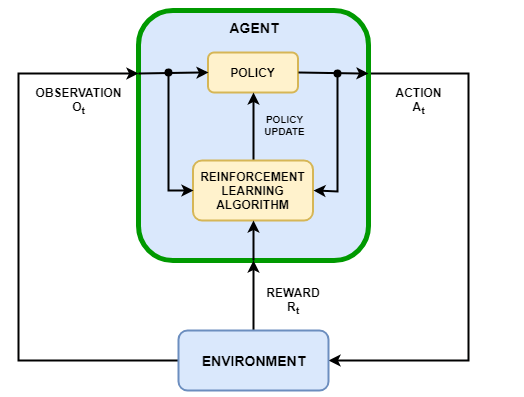
\includegraphics[width = 0.5\linewidth]{figures/MatlabRL.PNG}
    \caption{Rl Environment-Agent Interaction \cite{rl3}}
    \label{fig:my_label}
\end{figure}


\begin{enumerate}

    \item Construct a reset and step function that will be used to construct the environment in which the agent will be in.
    
    \item Define action and Observation information to define how the agent and environment will interact.

    \item The environment was achieved using \textit{rlFunctionenv()} which requires action and observation information as well as the step and reset function.

        \[\textsf{Environment =  rlFunctionenv(ActInf,ObsInf,Stepfunc,Resetfunc)}\]

    \item The agent was constructed using the \textit{rlACAgent()} with the same action and observation options. 
    
    \[\textsf{Agent =  rlACAgent(ActInf,ObsInf)}\]
    
    \item Training options are set Using \textit{rlTainingOptions()} which are used to evaluate the success of an agent, then Agent is trained using \textit{train()}
    
    \[\textsf{TrainingData =  train(Agent,Environment)}\]
    
    \item Agents with the highest cumulative reward are kept.
\end{enumerate} 
 
\clearpage

 \begin{wrapfigure}{r}{0.5\linewidth}
\begin{center}
    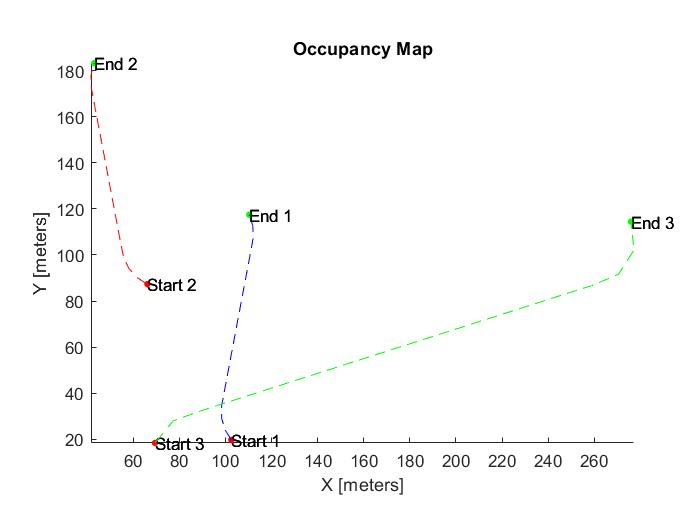
\includegraphics[width=0.45\textwidth]{figures/DroneInitial.jpg}
    \end{center}
    \caption{Environment initial conditions}
    \label{fig:Drone Initial}
\end{wrapfigure}

\subsection{Reset function}
The reset function initiates each episode. It sets the initial positions, velocity, acceleration and endpoints for n drones drone. Figure \ref{fig:Drone Initial} shows the environment 3 drone objects are created at random initial coordinates and 3 corresponding endpoints.

\subsection{Step Function}

\subsubsection{Actions}
From equations, \ref{equ:AtractiveForce}, \ref{equ:sep}, \ref{equ:al} and \ref{equ:coh} in section 2. The control input is the input force to the system so:

\[u_{i} = K_{a_i}\vec{V}_{E_i} + K_{s_i}\vec{V}_{SC_i} + K_{al_i}\vec{V}_{AlC_i} + K_{c_i}\vec{V}_{CD_i} - K_{d_i}\vec{V_i}\]
where:
\[{{\textbf{U}}}(t) = [u_1(t), u_2(t),..., u_N(t)]\]

\noindent
Control signal $U(t)$ is constructed with gains such that:


\begin{align*}
 K_i(t) &= 
    \begin{bmatrix*}[r]
        K_{a_i} & K_{s_i} & K_{al_i} & K_{c_i} & K_{d_i}\\
    \end{bmatrix*}
    V_i(t) = 
    \begin{bmatrix*}
        \vec{V}_{E_i}\\
        \vec{V}_{SC_i}\\
        \vec{V}_{AlC_i}\\
        \vec{V}_{CD_i}\\
        \vec{V}_{d_i}
    \end{bmatrix*}\\
    \centering
\end{align*}
   

where:


\begin{equation}
\begin{split}
    {{\textbf{A}}}(t) &= [K_1(t), K_2(t),..., K_N(t)]\\
    {{\textbf{V}}}(t) &= [V_1(t), V_2(t),..., V_N(t)]\\
    \end{split}
\end{equation}
The agent is able to change gains to vary the behaviour of the system, prioritising certain behaviours. $\textbf{A}(t)$ is the action at each step. The information is constructed using rlNumericSpec() which is used to set the action as a $5\times N$ array of continuous values such that:

\[\textsf{ActionInfo = rlNumericSpec([5 n]);}\]
\[\textsf{ActionInfo.LowerLimit = zeros(5,n)};\]
\[\textsf{ActionInfo.UpperLimit =  ones(5,n)*20;}\]

Reasonable Upper and lower limits were set based on other boid simulations parameters.
\subsubsection{Observations}
As actor-critic networks are a model free approach more than just states spaces can be observed. The observations made are the 5 desired velocities calculated from the boids model as well as position, endpoint and number of flock-mates. This is constructed as follows:

\[O_i = \{V^T_i,\vec{p}_i,\vec{p}_{end},j\in{\cal{F}}_i\}\]

where:

\[V^T_i = \Big[\vec{V}_{E_i}, \vec{V}_{SC_i}, \vec{V}_{AlC_i}, \vec{V}_{CD_i}, \vec{V}_{y_i}\Big]\]

These are all 2 dimensional vectors except for $j\in{\cal{F}}_i$ which is the number of flock-mates for agent i. The x and y coordinates are separated to give:

\[O_i = \Big[V_{E_{ix}}, V_{SC_{ix}}, V_{AlC_{ix}}, V_{CD_{ix}}, V_{d_{ix}}, p_{ix},p_{end_{ix}}, V_{E_{iy}}, V_{SC_{iy}}, V_{AlC_{iy}}, V_{CD_{iy}}, V_{d_{iy}},p_{iy},p_{end_{iy}},j\in{\cal{F}}_i\Big]\]

The full system observation at time step t is constructed as:

\[\textbf{O}(t) = [O_1(t),O_2(t),...O_N(t)]\]

This dimension is defined in MATLAB as:

\[\textsf{ObservationInfo = rlNumericSpec([15 n]})\]

\subsubsection{States: multi-agent  double integrator}
A Multi-agent double integrator model\cite{mul1}  was used to simulate environment dynamics. Let N drones be moving in a 2-Dimensional plane. The linear state-space representation of the double integrator model is then:

\begin{equation}
\begin{aligned}
\dot{\xi}_{i}(t) &= A\xi_i(t) + Bu_i(t)\\
v_{i}(t) &= C\xi_i(t)
\end{aligned}
\end{equation}

\noindent
Where $\xi_i = [x_i,\dot{x}_i,y_i,\dot{y}_i]^T$ and:

\vspace{0.5cm}


\begin{align*}
 A &= 
    \begin{bmatrix*}[r]
        0 & 1 & 0 & 0\\
        0 & 0 & 0 & 0\\
        0 & 0 & 0 & 1\\
        0 & 0 & 0 & 0
    \end{bmatrix*}
    B = 
    \begin{bmatrix*}
        0 & 0\\
        1 & 0\\
        0 & 0\\
        0 & 1
    \end{bmatrix*}\\
    \centering
    C &= 
     \begin{bmatrix*}
        1 & 0 & 0 & 0\\
        0 & 0 & 1 & 0
    \end{bmatrix*}
\end{align*}

\noindent
Here, $v_i$ is the measured output which in this case is the position $(x_i,y_i)$ of the $i^{th}$ drone. This is constructed using the perception radius from equation \ref{equ:per} section \ref{flock}. In this multi agent system agents are aware of relative speed:
\begin{equation}
z_{i}(t) = \sum_{j\in{\cal{F}}_i}(v_i(t) - v_j(t))
\end{equation}

\noindent
For $i = 1...N$, the flock consists of the set ${\cal{F}}_i \subset\{1,2,...N\}/\{i\}$.This then denotes the other drones that the agent $i$ is aware off. The system is:

\begin{equation}
\dot{X}(t)=(I_{N}\otimes A)X(t)+(I_{N}\otimes B)U(t)
\end{equation}

\noindent
where,

\begin{equation}
\begin{split}
    X(t) &= (\xi_1(t), \xi_2(t), ... \xi_N(t))\\
    U(t) &= (u_1(t), u_2(t), ... u_N(t))
    \end{split}
\end{equation}
\noindent
at the network level:
\begin{equation}
Z(t)=({\cal F}\otimes C)X(t)
\end{equation}


\subsection{Reward function}
The reinforcement learning objective from equation \ref{equ:re} section \ref{GOAL}:

\[J(\theta) = \mathbb{E}[\sum_{t=0}^{T-1} r_{t+1}]\]

The reward therefore needs to maximise in the direction of the desired emergent behaviour.\cite{rew1}.

\begin{itemize}
    \item \textbf{Step reward} provided at every step.
    \item \textbf{Episodic reward} is provided at the end of every simulation which occurs at once all agents have arrived or the maximum iterations have been reached. 
\end{itemize}

In this scenario it is the agent should move towards the destination but also flock with other agents as long as this does not sway it too much from its original objective. If the agents are only rewarded for discrete observations such as arriving at a destination or flocking with a member the reward system may be sparse, where the agent receives no signal for long series of actions and observations. To reduce the sparsity of reward, a continuous reward function is designed to push certain behaviours which is incorporated into the step reward function. \cite{shaping}
\clearpage
\subsection{Shaping step reward}
The function $e^{-k_r\sqrt{x^2}}$ is used to construct the reward function.

\begin{figure}[h]
        \centering
   \begin{subfigure}[b]{0.45\textwidth}
         \centering
         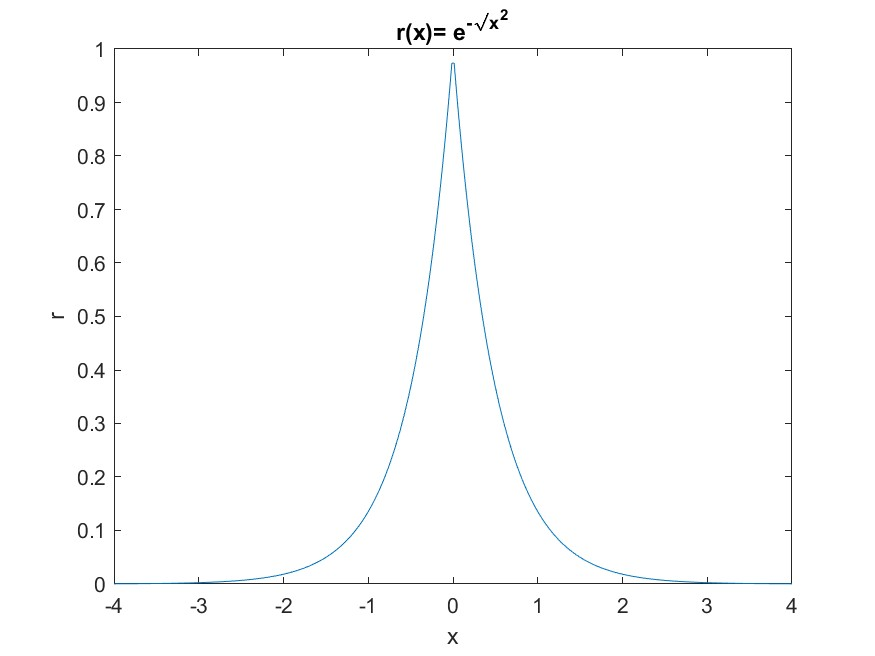
\includegraphics[width=\textwidth]{figures/Exp.jpg}
         \caption{Exponential decay 2D}
         \label{fig:exp1}
     \end{subfigure}
     \hfill
     \begin{subfigure}[b]{0.45\textwidth}
         \centering
         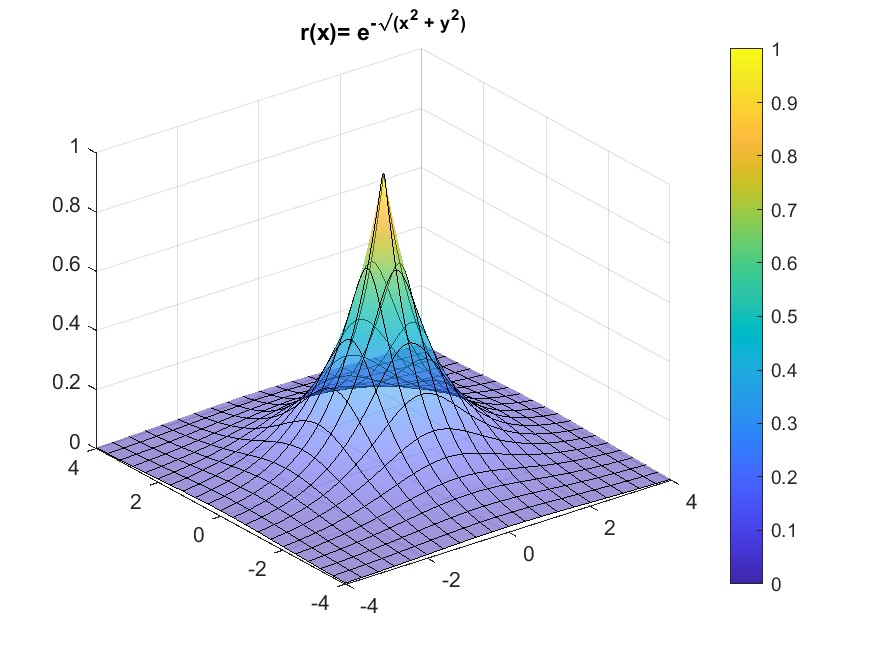
\includegraphics[width=\textwidth]{figures/Exp2.jpg}
         \caption{Exponential decay 3D function }
         \label{fig:exp2}
     \end{subfigure}
     \hfill
\end{figure}

As shown in figures \ref{fig:exp1} and \ref{fig:exp2}, The maximum reward is given at the roots of the function, which in this case are the coordinates of the agent, and tends to 0. This is ideal for a multi-agent system as it allows the control of the size of the horizon of influence of the agents with the constant $k_r$ which is found by applying constraints to the radius of effect and threshold.\hfill\vspace{0.5cm}\\

\noindent
Let the reward function for a point be:

\[r(x,y) = e^{-k_r\rho}\]


Where $\rho = \sqrt{(x-x_{pos})^2 + (y-y_{pos})^2}$. When agent coordinates are equal to the point coordinates:

\[e^0 = 1\]

The maximum area of effect is defined as $\rho_{max}$ and the threshold reward $r_t$ is the reward at $\rho = \rho_{max}$ so:

\[r_t = e^{-k_r\rho_{max}}\]

so:

\[k_r = \frac{ln(r_t)}{\rho_{max}}\]

The reward function of the drones is set to a smaller radius as it is only beneficial to flock when close to another agent. The maximum area of influence is expressed as relative to the size of the map by using the map hypotenuse $h = \sqrt{width^2 + height^2}$. The threshold was set to $r_t = 0.05$ as this meant the signal was only 5\% of the original signal at that point and so had a low effect on change in reward.\vspace{0.5cm}\\
\clearpage
\noindent
\textbf{Flocking reward}\\
\noindent
The flocking reward was chosen  so that the effective area of the drones needed to be smaller than the endpoint effective area so:
\[max(\rho_f) = 0.2h\]
then,
\[k_f = \frac{ln(0.05)}{0.2h}\]

The flocking reward is then the average of all flocking rewards thus,

\begin{equation}
    r_{f_{i}} = \frac{1}{n}\sum_{j=1}^{f} e^{-k_f\sqrt{({x}_i - {x}_j )^2 + ({y}_i - {y}_j)^2}}
    \label{equ:Frew}
\end{equation}


\noindent
\textbf{Endpoint Reward}

\[max(\rho_e) = 0.6h\]
so,
\[k_e = \frac{ln(0.05)}{0.6h}\]

\begin{equation}
    r_{e_i} = e^{-k_e\sqrt{({x}_i - {x}_e )^2 + ({y}_i - {y}_e)^2}}
    \label{equ:Erew}
\end{equation}

\noindent
The sum of these two reward functions is represented in figure \ref{fig:RewardFunc}. See appendix A1 for more details.

\begin{figure}[h]
  \begin{center}
    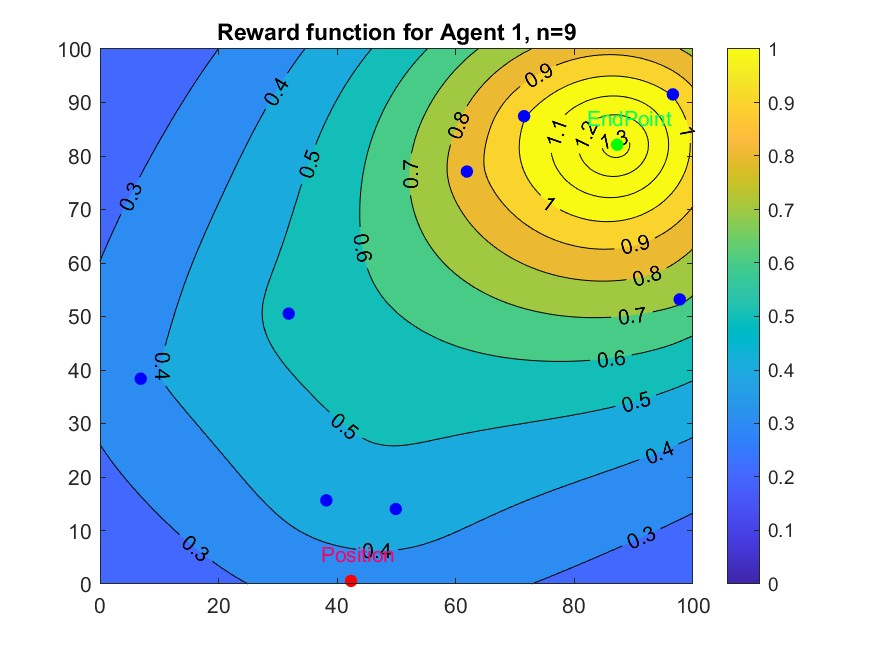
\includegraphics[width=0.60\textwidth]{figures/Reward.jpg}
    \end{center}
    \caption{Reward function with 9 agents}
    \label{fig:RewardFunc}
\end{figure}
\clearpage
\noindent
\textbf{Penalty}\newline
From equation \ref{equ:rew} cumulative return for time step k is:

\[r_t^\gamma = \sum_{k =  t}^T\gamma^{n-t}r(s_k,a_k)\]

If $0 < \gamma < 1$ and the $r > 0$ then it can be seen that $r^\gamma$ tends to 0. This implies the maximisation problem is impossible. To solve this, a penalty is added to the step function to push the agent to arrive within a set number of steps defined as $T_{max}$.  The exponential function $ae^{-k_{p}x}$ is used as constants a and $k_p$ can be changed to form the appropriate signal. For the agent to arrive within $T_{max}$ steps the following definition is formulated:
\begin{center}
    \(r_t = 0\) for \(t = T_{max}\)
\end{center}

Total step reward $r_t$ is the sum of equations \ref{equ:Frew} and \ref{equ:Erew} minus the penalty.

\[r_{t_i} = r_{f_i} + r_{e_i} - r_{p_i} = 0\]
where:
\[r_{p_i} = ae^{k_{p}T_{max}}\]
and maximum possible values for $r_{f_i}$ and $r_{e_i}$ is 1. Through substitution this yields:

\[ae^{k_{p} T_{max}} = 2\]

Applying initial conditions a is found:
\begin{center}
    \(ae^0 = a\) where a is set so that \(a << 2,\)
\end{center}


Applying terminal conditions:
\begin{equation}
    k_{p} = \frac{ln(\frac{2}{a})}{T_{max}}
    \label{equ:kp}
\end{equation}
Note that $r_{f_i}$ the sum of $r_{e_i}$ is only equal to 2 when all reward functions are at the same point which is unlikely. It is better to overestimate, however, as this prevents exponential growth of the reward.
\begin{figure}[h]
    \centering
    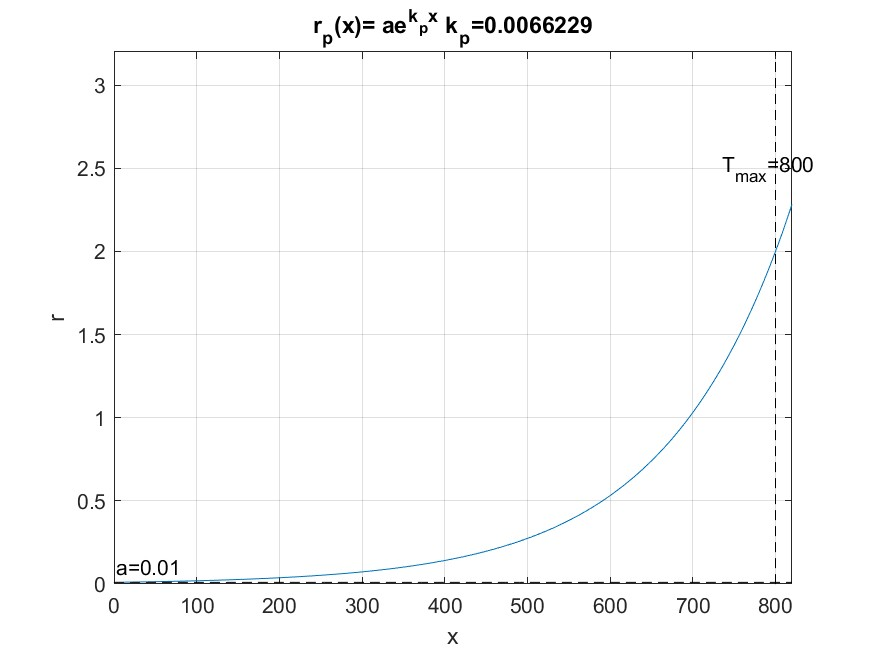
\includegraphics[width=0.4\textwidth]{figures/Exp3.jpg}
    \caption{Penalty function}
    \label{fig:exp3}
\end{figure}\\
Figure \ref{fig:exp3} shows the penalty function used. The reward for each agent step is then:
\[r_{t_i} = r_{f_i} + r_{e_i} - r_{p_i}\]

The total reward for each simulations time step $n$ is then the average reward of the N agents:
\[r_{step_n} = \frac{1}{N}\sum_{i=1}^{N}r_{t_i}\]


\subsection{Episodic reward}

The episodic reward takes into account the overall success of the simulation, providing this reward once a maximum number of steps is achieved or all agents have arrived at their destinations. This is represented as:

\[R_{total} = r_{episodic} + \sum^T_{n=1}{r_{step_n}}\]

The episodic reward is based of the terminal state of the system.
It takes number of individuals that have arrived at their destinations such that if agent i has arrived within a set arrival distance:
\[r_{a_i} = 1\]
And if agent i hasn't arrived:
\[r_{a_i} = 0\]

Then total episodic reward is 
\[r_{episodic} = \frac{1}{N}\sum_{i=1}^{N}r_{a_i}\]

The overall maximisation problem becomes:

\[MaxJ(\theta) = max(R_{total})\]










\subsection{Training Options}

Knowing the maximum cumulative reward that is achievable is important as it sets limits as to what outcome to expect. The reinforcement learning toolbox provides the \(rlTrainingOptions()\) allows us to define the criteria for a well-trained agent as well as limit the number of steps per episode.\\


\begin{center}
    \textsf{trainOpts = rlTrainingOptions('MaxStepsPerEpisode',800,...\\'SaveAgentCriteria','EpisodeReward','SaveAgentValue',800);}\\
\end{center}


\noindent
This limits the maximum number of steps per episode as well as specifies that an agent with a cumulative reward of \(J(\theta) = 1050\)  is a successful agent.
%----------------------------------------------------------------------------------------
%	THESIS CONTENT - APPENDICES
%----------------------------------------------------------------------------------------
%CHANGE FIGURE NO AGENT FLOCKING

\section{Results}
\subsection{No agent}
To provide a baseline for what flocking behaviour looks like figure \ref{fig:NoAgentFlocking} demonstrates flocking with constant gains for each step. the flocking can be seen to occur as drones are in proximity to each other and all drones are arriving at their individual destinations.

\begin{figure}[h]
  \begin{center}
    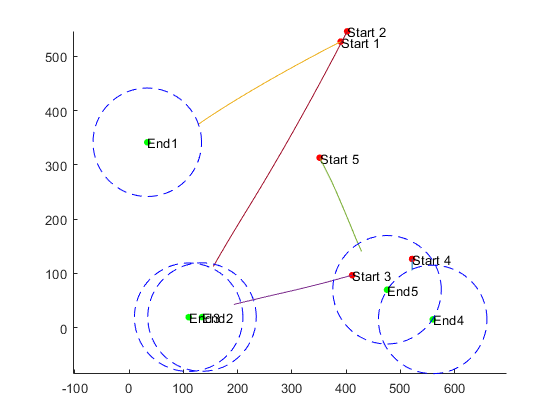
\includegraphics[width=0.4\textwidth]{figures/NoAgent.png}
    \end{center}
    \caption{No agent Flocking}
    \label{fig:NoAgentFlocking}
\end{figure}

\subsection{Agent training}
During the training, the agents would behave in a stochastic fashion to facilitate exploration. The training was stopped once a satisfactory average reward was achieved and the subsequent agents were saved.


\begin{figure}[h]
  \begin{center}
    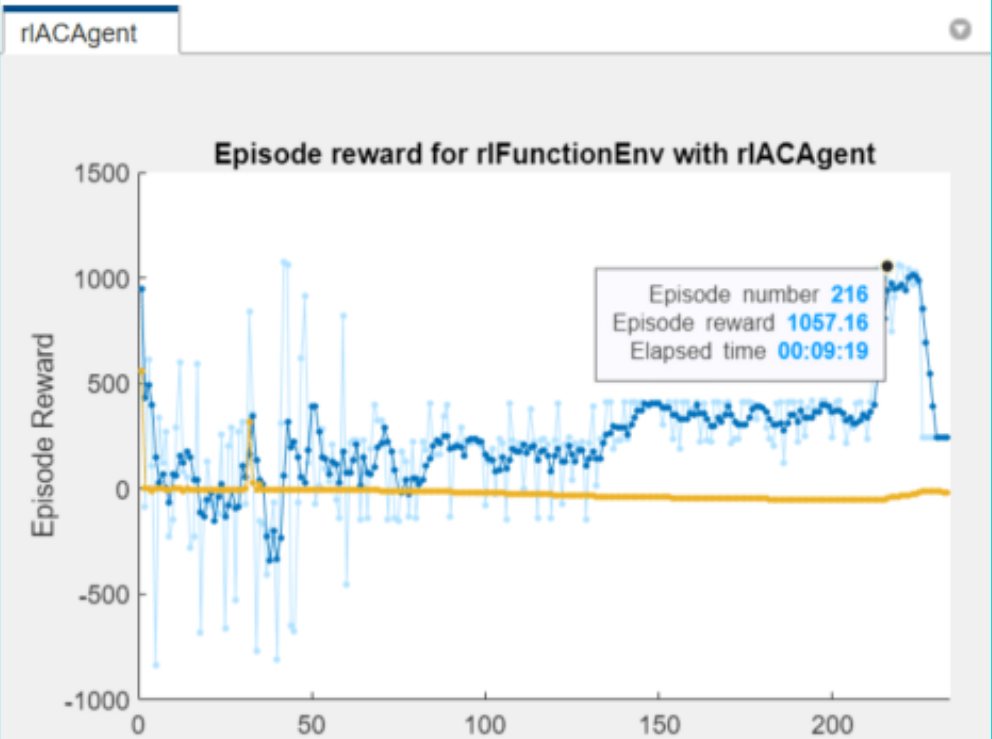
\includegraphics[width=0.4\textwidth]{figures/TrainingData.PNG}
    \end{center}
    \caption{Agent Training}
    \label{fig:Agent Training}
\end{figure}

Figure \ref{fig:Agent Training} demonstrates this training where 3 values are shown: episode reward, an average taking into account the last 5 episodes and the Q0 estimated reward. The average reward, calculated over the last 5 steps, steadily increases as the agent performs more episodes. The agent learns steadily until it reaches a certain amount of episodes and suddenly loses all its learned behaviour. This is a common issue in reinforcement learning classified as "catastrophic forgetting"\cite{cat1}. This might be corrected by varying the learning rate once a certain agent is achieved. This would mean the agent would have a more robust policy function although learn slower.

\subsection{Trained agent}
Once trained the agent behaves in a deterministic way as it has established the optimal policy function. This means for every state input the agent has a definite action to perform. The simulation is then repeatable as there is a definite action for every state. 

\begin{figure}[h]
  \begin{center}
    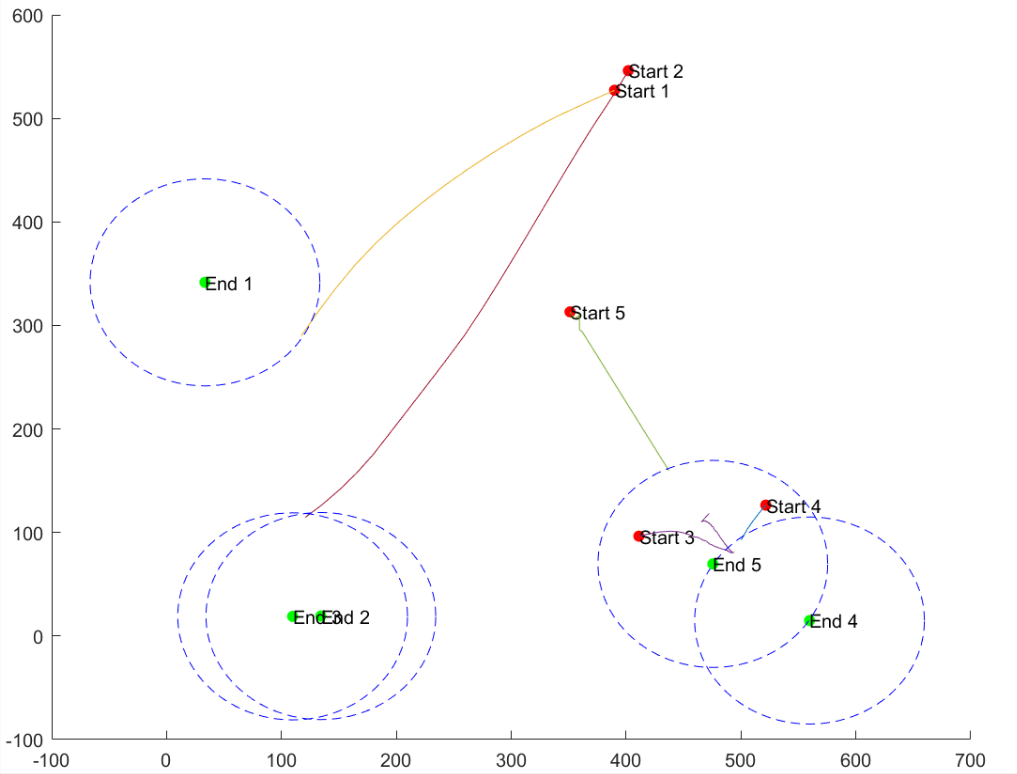
\includegraphics[width=0.6\textwidth]{figures/TrainedAgent.PNG}
    \end{center}
    \caption{Trained Agent}
    \label{fig:TrainedAgentFlocking}
\end{figure}

\subsection{Emergent Behaviour}
Emergent behaviour is a qualitative analysis that is useful in understanding how the reward affects agent behaviour. If certain undesirable behaviours emerge this is a sign that the reward function is promoting the wrong actions. From the trained agent’s performance in figure \ref{fig:TrainedAgentFlocking} some useful behaviours arise as well as some problematic behaviours:

\begin{itemize}
\item
Flocking is achieved which shows drones 1 and 2 arriving at designated locations from sides that benefit both members, this might be useful if multiple drones need to deliver packages but also avoid certain areas. 

\item
Some drones are not arriving at their destination which is a definite example of a scenario that is a detriment to the system. Drone 3 is choosing to flock with drones 4 and 5 rather than arrive at the destination. 

\end{itemize}
\clearpage
\section{Discussion}
The actions that the agent can perform are what determine how the agent controls the system. Providing the agent with a guidance system constrains the possibilities of actions it can take which has positive and negative influences on the system:\vspace{0.2cm}

\noindent
\textbf{+} The agent can learn quickly as there are fewer possible actions.\\

\noindent
\textbf{-}The agent is constrained to certain motions and is not given enough degrees of freedom the system lacks controllability.\cite{con2}\hfill\vspace{0.2cm}

\noindent
Since the first publication in 1987\cite{boid0}, the boid flocking behaviour has been iterated upon to provide the agent with the ability to learn new behaviours. These include having different perception radii for separation, alignment and cohesion, limiting the field of view of boids and allowing for flock leaders.\cite{boid1} These are just some examples of model variation that are possible. The application would be used to design the model. In the case of drones, lidar or some such sensor might be to detect the relative and heading of other UAVs. The simulation in this project uses a very simplistic model of the world. To reach further conclusions it would be desirable to further elaborate on the model.
The reward function here focuses on only 2  characteristics: The position of the drone and the number of steps  taken. The emergent behaviour exhibited by the drone is limited by this. Additional factors could be taken into account especially if the model representation expanded such as the power used to create a path.
In this case, the reward function promotes drone flocking as well as arriving at individual destinations within a limited number of steps in any scenario. This simulation is in 2 dimensions, so the altitude is not considered. This would obviously play a role in deciding whether to flock if a drone is at a certain altitude or is descending towards its destination.\\
Positive emergent behaviour was achieved in some sense so to continue down this path it is important to establish why it is being successful and how the reward function and overall machine learning structure can be leveraged to further improve the algorithm.

\subsection{Improvements}
To further encourage the positive emergent behaviour as well as discourage the issues that arise multiple factors come into play

\subsubsection{Machine learning structure}

The structure of learning can affect the learning speed of the agent but also be used to determine the application of the agent. The current machine learning structure uses a centralised agent that controls n drones, providing a [5, N] gain matrix at each iteration step controlling the swarm. Instead of this a multi-agent structure can be defined where each agent controls a single drone. This would simulate a decentralised network which is better suited to a multi-vehicle system.

\begin{itemize}
    \item 
    The application could work with drones that are not in communication with each other if there is sufficient sensor information about other drones. This structure would also mean the number of drones would no longer affect the dimensions of action and state matrices creating a more generalised agent. 
    \item
    Learning speed would increase as a result of agents learning in parallel, as for a simulation with N drones N agents would be trained as opposed to 1. To go even further 
    \item
    Agents could be assessed individually rather than taking a weighted sum of the overall reward. Agents could be removed from every simulation and the best ones could be used to seed the next generation of agents. This would improve the learning rate as well.
\end{itemize}

\subsubsection{Environment}
In this case, the environment is simplistic. There are no obstacles included as well as very simple environmental dynamics. The system could be represented in 3D and additional environmental characteristics could be included such as:

\begin{itemize}
    \item Differentiation of quad-copter\cite{quad1} and fixed-wing\cite{fix1} dynamics could be introduced to find how this affects the way they interact with each other.
    
    
    
    \item Consider benefits of flocking for efficiency for fixed-wing UAVs \cite{fix1}.
    
    \item Consider prevailing winds making use of head and tailwind.
    
\end{itemize}

\subsubsection{Optimisation}
Optimising the simulation is important in reinforcement learning as the more episodes that can be performed the more the agent can optimise its policy function. Code refactoring could be achieved through:

\begin{itemize}
    \item 
    Inclusion of a Quad-tree\cite{ref1}, which is a programming technique that compresses spacial data limiting the number of checks that need to be done when calculating whether agents are close to one another.
    \item
    Making use of specialised hardware that is optimised for RL\cite{ref2}.
    \item
    Using open AI platform to produce a better reinforcement learning structure.\cite{AI}
\end{itemize}



\subsubsection{Reward Function}
Being the key cause for emergent behaviour the reward function can be changed to take into account more of the environment. This clearly benefits from more in-depth environmental dynamics. The function that is used in this scenario is specifically tailored for the specific range. The reward function could be altered in many ways depending on the intended application, here are some possibilities:

\begin{itemize}
    \item 
    Make reward for position relative to the range that it will be used to make more general emergent behaviour.
    
    \item
    Include altitude in the 3-dimensional environment
    
    \item Include additional penalty for position, namely no fly-zones \cite{res1}.
\end{itemize}

 
\section{Conclusion}
It has been demonstrated that by layering boid flocking behaviour and potential field functions a reinforcement learning agent can be trained to achieve emergent flocking behaviour which could be used to control drone traffic. Although the simulation is simplistic and the machine learning structure may not be optimal, this shows a basic framework is scale-able and could be layered with other reward functions to achieve more complex emergent behaviour.

\subsection{Suggestions for further work}
For further development of this idea one could look at how this system could be scaled further by using a further customised reinforcement learning algorithm. The loss function in this case is quite basic and therefore limits the learning capabilities. Using the Resources available on open AI make it easier to design a capable RL environment to suit specific requirements.\cite{AI} Making use of a Multi-Agent Particle Environment style of RL might also improve learning speeds and scale-ability.\cite{MPE} 

By simulating the environment in 3 dimensions and the addition of obstacles in the form of a city block plan could be used to emulate an environment closer to that intended for the agent.

\clearpage % start appendices on a new page

\begin{thebibliography}{9}
\addcontentsline{toc}{section}{References}

\bibitem{boid0}
\textit{Reynolds, C.W. (1987) Flocks, Herds and Schools: A Distributed Behavioral Model. ACM Siggraph Computer Graphics, 21, 25-34.}

\bibitem{boid1}
Craig W. Reynolds,\\
\textit{“Boids (Flocks, Herds, and Schools: A Distributed Behavioral
Model).” Red3d.com, 2019, www.red3d.com/cwr/boids/.}

\bibitem{boid2}
Bajec, I. Lebar, et al.\\
The computational beauty of flocking: boids revisited
\textit{“The Computational Beauty of Flocking: Boids Revisited.” Mathematical and Computer Modelling of Dynamical Systems, vol. 13, no. 4, Aug. 2007, pp. 331–347, 10.1080/13873950600883485. Accessed 15 June 2021.}

\bibitem{boid3}
A.V. Moere,\\
Time-Varying Data Visualization Using Information Flocking Boids,\hfill\\
\textit{  " IEEE Symposium on Information Visualization, 2004, pp. 97-104, doi: 10.1109/INFVIS.2004.65.}

\bibitem{boid4}
Craig W. Reynolds
Steering Behaviors For Autonomous Characters
\textit{Www.red3d.com, www.red3d.com/cwr/steer/gdc99/}

 \bibitem{mult1} Qu, Guannan. “Scalable Multi-Agent Reinforcement Learning for Networked Systems with Average Reward.” 
 
 \bibitem{shaping}
 Adam Daniel Laud
Theory and Application of Reward Shaping in Reinforcement learning

%DroneCompanies
\bibitem{com1}
Drone Up,\\
\textit{“Let’s Fly! | DroneUp.” www.droneup.com/.} 

\bibitem{com2}
Wing,\\
Owned by Google,\\
\textit{Wing. wing.com/.}

\bibitem{com3}
“DHL Drone Delivery and Parcelcopter Technology\\
\textit{Discover DHL.” Dhl.com, 2022, \\ www.dhl.com/discover/en-my/business/business-ethics//parcelcopter-drone-technology.\hfill}

\bibitem{com4}
Skyopener Project.\\
\textit{M3 Systems, m3systems.eu/en/skyopener-project/. Accessed 16 Apr. 2022.} 

%Drone efficiency
\bibitem{eff1}
Kirschstein, Thomas. \\
\textit{“Comparison of Energy Demands of Drone-Based and Ground-Based Parcel Delivery Services.” Transportation Research Part D: Transport and Environment, vol. 78, 1 Jan. 2020, p. 102209, www.sciencedirect.com/science/article/pii/S1361920919309575, 10.1016/j.trd.2019.102209. Accessed 17 Mar. 2020.} 

\bibitem{eff2}
Gulden, Timothy R.\\
The Energy Implications of Drones for Package Delivery,\\ 
\textit{The Energy Implications of Drones for Package Delivery: A Geographic Information System Comparison. Santa Monica, CA: RAND Corporation, 2017.}

%Drone Restricted Zones
\bibitem{res1}
NO FLY DRONES\\
\textit{“No Fly Drones.” No Fly Drones, www.noflydrones.co.uk/.} 

%Drone Range
\bibitem{far1}
NEXTECH\\
\textit{“VTOL Vertical Take off and Landing Drone.” Nextechnology,\\ shop.airbornedrones.co/products/vtol-drone. Accessed 16 Apr. 2022.}

\bibitem{far2}
DJI\\
\textit{“Mavic 3 - Specs - DJI.” DJI Official, www.dji.com/uk/mavic-3/specs.} 

%Drone Terrorism
\bibitem{ter1}
ASSOCIATION OF THE UNITED STATES ARMY\\
\textit{“The Role of Drones in Future Terrorist Attacks.” AUSA, 26 Feb. 2021,\\ www.ausa.org/publications/role-drones-future-terrorist-attacks.} 

\bibitem{ter2}
Yaacoub, Jean-Paul, and Ola Salman.\\
 “Security Analysis of Drones Systems: Attacks, Limitations, and Recommendations.”\\
\textit{Internet of Things, May 2020, p. 100218,\\ www.ncbi.nlm.nih.gov/pmc/articles/PMC7206421/, 10.1016/j.iot.2020.100218.}

\bibitem{ter3}
D-fend\\
\textit{“Drone Threat, Counter Drone.” D-Fend Solutions,\\ www.d-fendsolutions.com/drone-threat-overview/. Accessed 16 Apr. 2022.}

\bibitem{ter4}
Seongjoon Park et al.\\
\textit{Park, Seongjoon, et al. “Survey on Anti-Drone Systems: Components, Designs, and Challenges.” IEEE Access, vol. 9, 2021, pp. 42635–42659, 10.1109/access.2021.3065926.}

%Flocking
\bibitem{flo1}
Chao Yan et al.\\
\textit{Yan, Chao, et al. “Fixed-Wing UAVs Flocking in Continuous Spaces: A Deep Reinforcement Learning Approach.” Robotics and Autonomous Systems, vol. 131, Sept. 2020, p. 103594, 10.1016/j.robot.2020.103594.}
%Neural networks and actor critic
\bibitem{neu1}
Understanding Actor Critic Methods and A2C\\
\textit{Yoon, Chris. “Understanding Actor Critic Methods.” Medium, 17 July 2019,\\ towardsdatascience.com/understanding-actor-critic-methods-931b97b6df3f.},

\bibitem{neu2}
Deriving Policy Gradients and Implementing REINFORCE\\
\textit{Yoon, Chris. “Deriving Policy Gradients and Implementing REINFORCE.” Medium, 23 May 2019, medium.com/@thechrisyoon/deriving-policy-gradients-and-implementing-reinforce-f887949bd63.},

%Perceptron
\bibitem{per1}
Perceptron,\\
Brilliant Math \& Science Wiki.”\\
\textit{“ Brilliant.org, brilliant.org/wiki/perceptron/\#:~:text=The\%20perceptron\%20is\%20a\%20machine.}
%Deep learning
\bibitem{deep1}
Charu C. Aggarwal,\\
\textit{Machine Learning with Shallow Neural Networks. In: Neural Networks and Deep Learning. Springer, Cham.},
(2018).

\bibitem{deep2}
Deep Learning and the Game of Go\\
\textit{Pumperla, Max, and Kevin Ferguson. Deep Learning and the Game of Go. Shelter Island, Ny, Manning Publications Co, 2019.}

%Reinforcement learning
\bibitem{rl1}
Sutton, Richard S,\\
\textit{ and Andrew Barto. Reinforcement Learning : An Introduction. Cambridge, Ma ; Lodon, The Mit Press, 2018.}

\bibitem{rl2}
Grondman, Ivo, et al.\\
\textit{ “A Survey of Actor-Critic Reinforcement Learning: Standard and Natural Policy Gradients.” IEEE Transactions on Systems, Man, and Cybernetics, Part c (Applications and Reviews), vol. 42, no. 6, Nov. 2012, pp. 1291–1307, 10.1109/tsmcc.2012.2218595. Accessed 27 Feb. 2020.}

\bibitem{rl3}
“Create MATLAB Reinforcement Learning Environments - MATLAB \& Simulink.”\\
\textit{www.mathworks.com/help/reinforcement-learning/ug/create-matlab-environments-for-reinforcement-learning.html.\hfill}
%Control
\bibitem{con1}
Stengel, Robert F.\\
Optimal Control and Estimation.\\
\textit{ Google Books, Courier Corporation, 20 Sept. 1994,\\ books.google.co.uk/books?hl=en\&lr=\&id=byRgDwAAQBAJ\&oi=fnd\&pg=PA1\&dq=Stengel\\+Optimal+Control+and+Estimation. Accessed 16 Apr. 2022.}

\bibitem{con2}
Control Systems/Controllability and Observability,\\
Wikibooks, Open Books for an Open World.” \\
\textit{En.wikibooks.org, en.wikibooks.org/wiki/Control\_Systems/Controllability\_and\_Observability\\\#:~:text=The\%20concept\%20of\%20controllability\%20refers.}

%Example visualisations
\bibitem{ex1}
“Boids Algorithm.\\
\textit{” Eater.net, eater.net/boids.},

%Code Help
\bibitem{cod1}
“The Nature of Code.”\\
\textit{ Natureofcode.com, natureofcode.com/book/chapter-6-autonomous-agents/.}

\bibitem{cod2}
“The Nature of Code.”\\
\textit{ Natureofcode.com, natureofcode.com/.}

\bibitem{mon1}
Metropolis, Nicholas, and S. Ulam.\\
\textit{ “The Monte Carlo Method.” Journal of the American Statistical Association, vol. 44, no. 247, Sept. 1949, pp. 335–341, 10.1080/01621459.1949.10483310.}

\bibitem{mar1}
Littman, M. L.\\
“Markov Decision Processes.”\\
\textit{ ScienceDirect, Pergamon, 1 Jan. 2001,\\ www.sciencedirect.com/science/article/pii/B0080430767006148.}

\bibitem{ac1}
Fujimoto, Scott, et al.\\
\textit{Addressing Function Approximation Error in Actor-Critic Methods.}


\bibitem{ac2}
Silver, David, et al.\\
\textit{ Deterministic Policy Gradient Algorithms.}

\bibitem{bel1}
TORRES.AI, Jordi.\\
“The Bellman Equation.”\\
The Bellman Equation\\
\textit{ Medium, 15 June 2020, towardsdatascience.com/the-bellman-equation-59258a0d3fa7.}


\bibitem{bel2}
\textit{“Bellman Optimality Equation in Reinforcement Learning.” Analytics Vidhya, 13 Feb. 2021, www.analyticsvidhya.com/blog/2021/02/understanding-the-bellman-optimality-equation-in-reinforcement-learning/\#:~:text=The\%20Optimal\%20Value\%20Function\%20is. Accessed 16 Apr. 2022.}

\bibitem{td1}
Hood, Jordan J.\\
“Reinforcement Learning: Temporal Difference (TD) Learning.”\\
\textit{www.lancaster.ac.uk/stor-i-student-sites/jordan-j-hood/2021/04/12/reinforcement-learning-temporal-difference-td-learning/.}

\bibitem{mul1}
Deshpande, Paresh, et al.\\
Formation Control of Multi-Agent Systems with Double Integrator Dynamics Using Delayed Static Output Feedback.”\\
\textit{ “ IEEE Xplore, 1 Dec. 2011, ieeexplore.ieee.org/document/6161074/figures\#figures. Accessed 16 Apr. 2022.}

\bibitem{rew1}
Brummerloh, Daniel.\\
“Ultimate Guide for AI Game Creation Part 2 — Training.”\\
\textit{ Medium, 7 Jan. 2021, towardsdatascience.com/ultimate-guide-for-ai-game-creation-part-2-training-e252108dfbd1. Accessed 16 Apr. 2022.}


\bibitem{mtl1}
“Create MATLAB Reinforcement Learning Environments - MATLAB \& Simulink.”\\
\textit{ Www.mathworks.com, www.mathworks.com/help/reinforcement-learning/ug/create-matlab-environments-for-reinforcement-learning.html. Accessed 16 Apr. 2022.}

\bibitem{cat1}
Cahill, Andy. \\
“Catastrophic Forgetting in Reinforcement-Learning Environments.”\\
\textit{ Ourarchive.otago.ac.nz, 2011, ourarchive.otago.ac.nz/handle/10523/1765. Accessed 16 Apr. 2022.}

\bibitem{lex1}
Fridman, Lex.\\
“MIT Deep Learning Basics: Introduction and Overview.”\\
\textit{ YouTube, 11 Jan. 2019, www.youtube.com/watch?v=O5xeyoRL95U.}

\bibitem{quad1}
“Dynamics Modeling of a Highly-Maneuverable Fixed-Wing UAV.”\\
\textit{ Researchgate, Apr. 2013, www.researchgate.net/publication/264773227\_Dynamics\_Modeling\_of\_a\_Highly-Maneuverable\_Fixed-Wing\_UAV.}

\bibitem{fix1}
“Accurate Simulator for Motion of the Quadcopter; Assuming Dynamic and Aerodynamic Effects.”\\
\textit{ Esearchgate, Apr. 2019, www.researchgate.net/publication/332980824\_Accurate\_Simulator\_for\_Motion\_of\_the\_Quadcopter\_Assuming\_Dynamic\_and\_Aerodynamic\_Effects.}

\bibitem{ref1}
Yin, Xiang, et al.\\
“Quadtree Representation \& Compression of Spatial Data.”\\
\textit{ Www.semanticscholar.org,\\ www.semanticscholar.org/paper/Quadtree-Representation-\%26-Compression-of-Spatial-Yin-Diintsch/d45d7f7d8817170ee0f9cec2db083a4852848621?p2df.}

\bibitem{ref2}
Shiri, Aidin, et al.\\
“Energy-Efficient Hardware for Language Guided Reinforcement Learning.”\\
\textit{ Proceedings of the 2020 on Great Lakes Symposium on VLSI, 7 Sept. 2020, eehpc.csee.umbc.edu/publications/pdf/2020/2020\_GLSVLSI\_RL\_Structured\_Language.pdf, 10.1145/3386263.3407652. Accessed 16 Apr. 2022.}

 \bibitem{AI}
 https://openai.com/api/
 
  \bibitem{MPE}
 Huichu Zhang Shanghai Jiao Tong University Shanghai, et al. “CityFlow: A Multi-Agent Reinforcement Learning Environment for Large Scale City Traffic Scenario: The World Wide Web Conference.” ACM Other Conferences, 1 May 2019, https://dl.acm.org/doi/abs/10.1145/3308558.3314139?casa\_token=nbe2mKJTQcEAAAAA\%3AJsYLiuBcf2e-DQ4YFfC0WLX0CRlDuj1UJnyeUpdcFouJDvfeosKk64t08rUAfQKStvFnwPB0Ieg. 
\end{thebibliography}
\clearpage % start appendices on a new page
\appendix % Cue to tell LaTeX that the following "chapters" are Appendices

% Include the appendices of the thesis as separate files from the Appendices folder
% Uncomment the lines as you write the Appendices

\include{Appendix}

%----------------------------------------------------------------------------------------
%	BIBLIOGRAPHY
%----------------------------------------------------------------------------------------

%\printbibliography[heading=bibintoc]

%----------------------------------------------------------------------------------------

\end{document}  

